\documentclass[11pt,a4paper]{article}

\usepackage[margin=0.78in]{geometry}
\usepackage[T1]{fontenc}
\usepackage[utf8]{inputenc}
\usepackage{lmodern}
\usepackage{graphicx}
\usepackage{booktabs}
\usepackage{array}
\usepackage{xcolor}
\usepackage{hyperref}
\usepackage{float}
\usepackage{caption}
\usepackage{enumitem}
\usepackage{titlesec}
\usepackage{tcolorbox}
\usepackage{tikz}
\usetikzlibrary{arrows.meta,positioning}

\graphicspath{{../figures/}}

\definecolor{snseteal}{HTML}{0E6B5C}
\definecolor{snseblue}{HTML}{1F4E79}
\definecolor{snseamber}{HTML}{D89000}
\definecolor{lightteal}{HTML}{E6F4F1}
\definecolor{lightblue}{HTML}{EAF1F8}
\definecolor{lightamber}{HTML}{FFF4DD}
\definecolor{darkgray}{HTML}{333333}

\hypersetup{
  colorlinks=true,
  linkcolor=snseblue,
  urlcolor=snseteal,
  citecolor=snseblue
}

\titleformat{\section}
  {\large\bfseries\color{snseblue}}
  {\thesection}{0.6em}{}
\titleformat{\subsection}
  {\normalsize\bfseries\color{snseteal}}
  {\thesubsection}{0.6em}{}

\setlist[itemize]{leftmargin=1.2em,itemsep=0.18em,topsep=0.18em}
\setlength{\parskip}{0.35em}
\setlength{\parindent}{0pt}

\newtcolorbox{findingbox}[1]{
  title=\textbf{#1},
  colback=lightteal,
  colframe=snseteal,
  boxrule=0.8pt,
  arc=2mm
}

\newcommand{\metriccard}[3]{%
  \fcolorbox{snseblue}{#1}{%
    \begin{minipage}[c][1.0cm][c]{0.29\linewidth}
      \centering
      {\large\bfseries #2}\\[-0.1em]
      {\small #3}
    \end{minipage}
  }%
}

\begin{document}

\begin{titlepage}
  \centering
  \vspace*{0.9cm}
  {\Large\bfseries\color{snseblue} Predicting Band Gaps of SnSe-Based Materials from Composition\par}
  \vspace{0.35cm}
  {\large FDP Capstone Project: Machine Learning for Materials and Metallurgical Engineering\par}
  {\large IIT (BHU), UGC MM-TTP, 13--18 July 2026\par}
  \vfill
  \begin{tabular}{>{\bfseries}p{0.32\linewidth}p{0.52\linewidth}}
    Project type & Composition-only materials-property prediction \\
    Data source & Materials Project \\
    Feature method & matminer Magpie composition descriptors \\
    Main model & Random Forest classifier and regressor \\
    Repository & \url{https://github.com/ShahiDDU/snse-bandgap-ml-capstone} \\
  \end{tabular}
  \vfill
  \metriccard{lightblue}{192}{cleaned compounds}
  \hfill
  \metriccard{lightteal}{132}{composition features}
  \hfill
  \metriccard{lightamber}{0.357 eV}{CV MAE}
  \vspace*{1.2cm}
\end{titlepage}

\section*{Executive Summary}

This capstone project builds a fast composition-only screening model for Sn--Se-based compounds. Materials Project returned 220 raw Sn--Se-containing entries; cleaning by formula and band-gap availability left 192 unique compounds. Each formula was converted into 132 Magpie composition descriptors using matminer. A Random Forest classifier distinguished metals from insulators with \(80.2\% \pm 3.7\%\) 5-fold cross-validated accuracy. For insulating compounds, a Random Forest regressor predicted band gap with MAE \(=0.357 \pm 0.072\) eV and \(R^2 = 0.401 \pm 0.168\). The most important regression feature was the range of electronegativity across the elements in the compound.

\section{Problem Statement}

SnSe is a narrow-gap IV--VI chalcogenide that has attracted strong interest for thermoelectric and electronic applications. Its useful behavior depends strongly on electronic structure, carrier type, crystal structure, and doping. Literature reports show that SnSe has high thermoelectric performance and that its band gap can be tuned by doping or electronic modification \cite{zhao2014,zhang2018}.

The project question is:

\begin{findingbox}{Research question}
Can a composition-only machine learning model predict whether a Sn--Se-based compound is a metal or an insulator, and for insulating compounds predict the Materials Project computed band gap?
\end{findingbox}

The practical motivation is screening. A model that only needs a chemical formula can rank candidate dopants or alloy compositions before slower calculations or experiments are attempted.

\section{Dataset}

The dataset was obtained from Materials Project using the \texttt{mp-api} Python client. Materials Project documents the use of \texttt{mp-api} as its supported Python route for accessing database data \cite{mpapi}. The query selected compounds containing both Sn and Se, with two to seven elements, and requested material ID, formula, and band gap.

\begin{itemize}
  \item Raw entries queried: 220.
  \item Cleaned dataset: 192 unique formulas with available band gap.
  \item Classification target: metal if band gap \(=0\), insulator if band gap \(>0\).
  \item Regression target: band gap in eV for insulators only.
  \item Class balance: 136 insulators and 56 metals.
\end{itemize}

\begin{figure}[H]
  \centering
  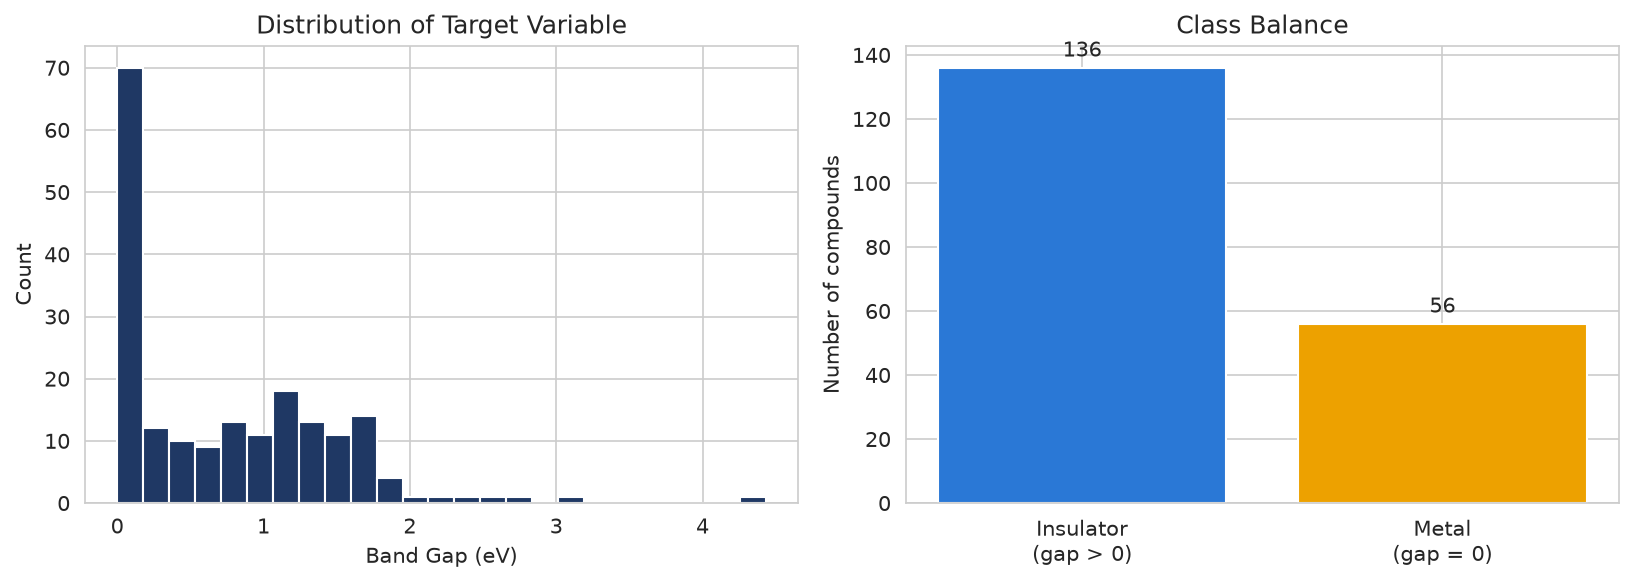
\includegraphics[width=0.95\linewidth]{fig_eda.png}
  \caption{Exploratory data analysis: band-gap distribution and metal/insulator class balance.}
  \label{fig:eda}
\end{figure}

\section{Feature Engineering}

The model uses composition only. No crystal-structure files, CIF files, atom positions, or local coordination descriptors were used. Each formula was parsed using pymatgen, which provides standard Python objects for compositions and structures \cite{pymatgen}. Then matminer generated Magpie composition descriptors. matminer is designed to transform materials information into numerical descriptors usable by downstream machine learning libraries \cite{matminer}.

Examples of generated descriptors include:

\begin{itemize}
  \item average and range of electronegativity;
  \item atomic radius statistics;
  \item valence-electron statistics;
  \item periodic-table column statistics;
  \item melting-temperature statistics.
\end{itemize}

\begin{center}
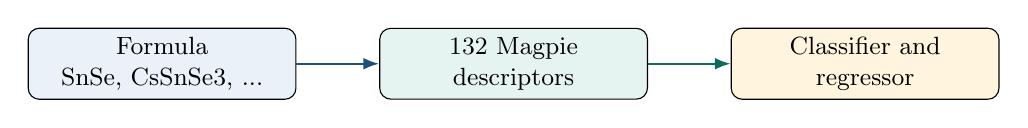
\begin{tikzpicture}[node distance=1.05cm, every node/.style={font=\small,align=center}]
  \node[draw,rounded corners,fill=lightblue,minimum width=3.4cm,minimum height=0.75cm] (formula) {Formula\\SnSe, CsSnSe3, ...};
  \node[draw,rounded corners,fill=lightteal,minimum width=3.4cm,minimum height=0.75cm,right=of formula] (desc) {132 Magpie\\descriptors};
  \node[draw,rounded corners,fill=lightamber,minimum width=3.4cm,minimum height=0.75cm,right=of desc] (model) {Classifier and\\regressor};
  \draw[-{Latex[length=2mm]},thick,snseblue] (formula) -- (desc);
  \draw[-{Latex[length=2mm]},thick,snseteal] (desc) -- (model);
\end{tikzpicture}
\end{center}

\section{Method}

Two linked models were trained:

\begin{enumerate}
  \item \textbf{Classification:} metal vs. insulator, comparing Logistic Regression and Random Forest.
  \item \textbf{Regression:} band-gap prediction for insulating compounds using Random Forest regression.
\end{enumerate}

Random Forest was selected as the main model because it can model nonlinear relationships and provides feature importance. scikit-learn describes Random Forest as an ensemble of decision trees trained on subsamples and averaged to improve prediction and reduce overfitting \cite{sklearnrf}.

Because the dataset is small relative to the 132 descriptors, the report uses 5-fold cross-validation as the primary evaluation method. This gives a more stable estimate than one train/test split.

\section{Results}

\subsection{Classification}

The Random Forest classifier achieved the best cross-validated classification accuracy.

\begin{table}[H]
\centering
\caption{Metal vs. insulator classification performance.}
\begin{tabular}{lcc}
\toprule
Model & Single split accuracy & 5-fold CV accuracy \\
\midrule
Logistic Regression & reported in notebook & \(78.1\% \pm 6.5\%\) \\
Random Forest & 84.6\% & \(80.2\% \pm 3.7\%\) \\
\bottomrule
\end{tabular}
\end{table}

The single-split confusion matrix showed that the model captured most insulators but was weaker for the smaller metal class. This is expected because the dataset contains more insulators than metals.

\subsection{Regression}

The Random Forest regressor predicted the band gap of insulating compounds with cross-validated MAE \(=0.357 \pm 0.072\) eV and \(R^2 = 0.401 \pm 0.168\).

\begin{figure}[H]
  \centering
  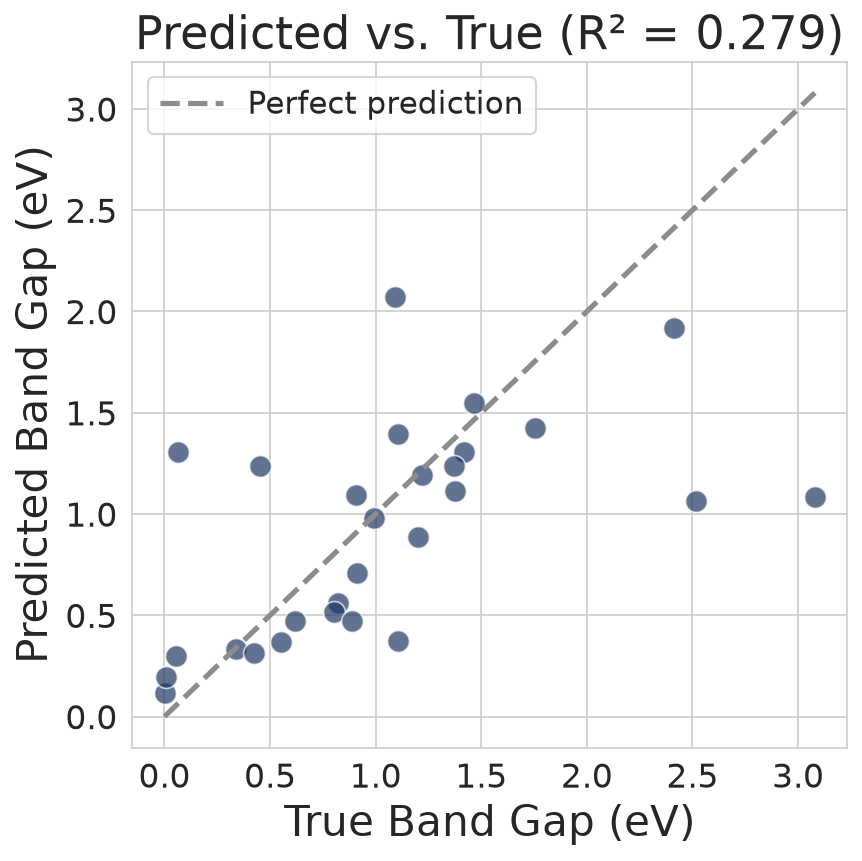
\includegraphics[width=0.62\linewidth]{fig_predictions.png}
  \caption{Predicted vs. true band gap for the Random Forest regressor on the held-out split.}
  \label{fig:pred}
\end{figure}

The plot shows useful correlation but also visible underprediction for some larger-gap compounds. This supports using the model as a first-pass screen, not as a replacement for higher-fidelity calculation.

\subsection{Feature importance}

\begin{figure}[H]
  \centering
  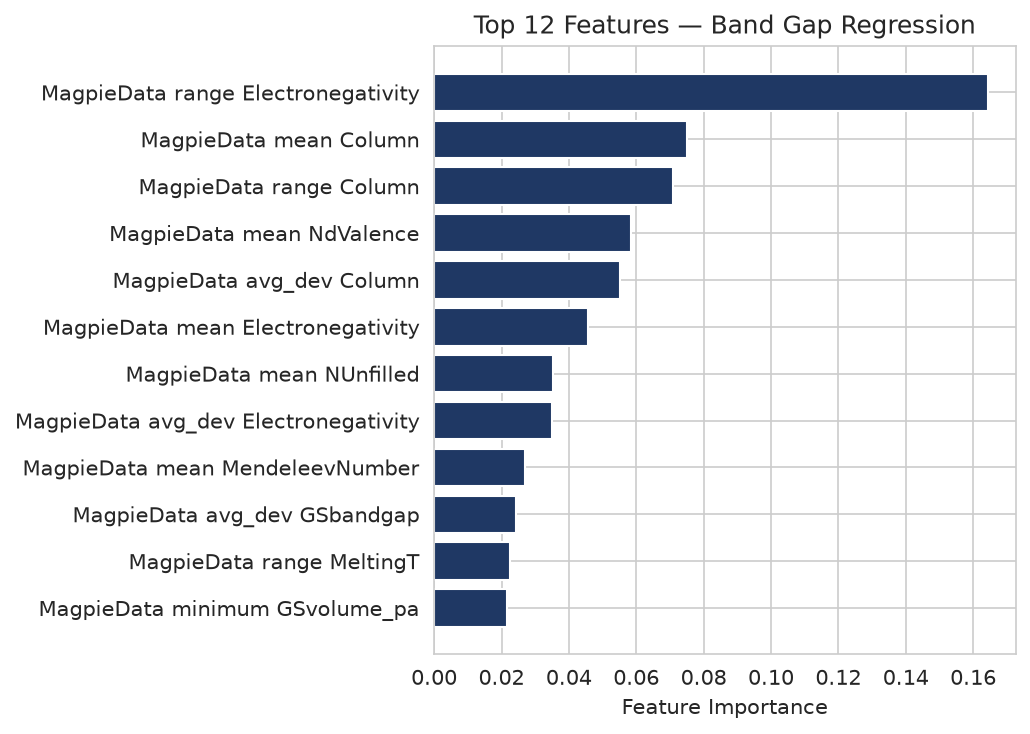
\includegraphics[width=0.78\linewidth]{fig_importance.png}
  \caption{Top 12 features for Random Forest band-gap regression.}
  \label{fig:importance}
\end{figure}

The most important descriptor was the range of electronegativity across elements in the formula. This is physically reasonable: large electronegativity differences influence bonding character and charge separation, which are closely related to band-gap formation. Feature importance should be interpreted as predictive importance, not proof of causation.

\section{Discussion}

The project demonstrates that a formula-only model contains useful information for Sn--Se-based materials. The Random Forest classifier improved over a simple linear model and gave more consistent cross-validation. The regression model captured a meaningful part of band-gap variation, but the \(R^2\) value shows that composition alone does not explain everything.

The main scientific message is conservative:

\begin{findingbox}{Main interpretation}
Composition-only descriptors can provide a fast screening signal for Sn--Se-based compounds, but they do not replace DFT calculations, structural analysis, or experiments.
\end{findingbox}

\section{Limitations and Next Steps}

\begin{itemize}
  \item \textbf{Composition-only limitation:} two polymorphs with the same formula receive identical features, even if their structures and band gaps differ.
  \item \textbf{Small dataset:} 192 compounds is modest compared with 132 features.
  \item \textbf{Class imbalance:} insulators are more common than metals, so accuracy must be interpreted carefully.
  \item \textbf{Computed target:} the target is Materials Project computed band gap, not direct experimental measurement.
\end{itemize}

Next steps would be to add structure descriptors, include related IV--VI chalcogenides such as SnS, SnTe, PbSe, PbS, PbTe, GeSe, GeS, and GeTe, and compare more models with repeated cross-validation.

\section{Conclusion}

This capstone project produced a complete workflow: database query, cleaning, composition featurization, classification, regression, cross-validation, feature-importance analysis, and scientific interpretation. The best model achieved \(80.2\% \pm 3.7\%\) classification accuracy and \(0.357 \pm 0.072\) eV regression MAE. The result is useful for fast screening and learning the materials machine learning workflow, while the limitations show why structure-aware modeling is the natural next step.

\section{Individual Contributions}

\begin{itemize}
  \item Group Leader and Modeling Lead: chose topic and dataset, coordinated workflow, built and ran the notebook.
  \item Data Lead: sourced and queried the Materials Project dataset.
  \item Preprocessing Lead: cleaned the data and built the feature pipeline.
  \item Report Lead: wrote and formatted the report.
  \item Presentation Lead: built the slide deck and prepared the presentation.
\end{itemize}

\begin{thebibliography}{9}

\bibitem{zhao2014}
Zhao, L.-D. et al. (2014).
\newblock Ultralow thermal conductivity and high thermoelectric figure of merit in SnSe crystals.
\newblock \emph{Nature}.

\bibitem{zhang2018}
Zhang, K. et al. (2018).
\newblock Widely tunable band gap in a multivalley semiconductor SnSe by potassium doping.
\newblock arXiv:1805.11248.

\bibitem{mpapi}
Materials Project Documentation.
\newblock Using the API.
\newblock \url{https://docs.materialsproject.org/downloading-data/using-the-api}

\bibitem{pymatgen}
pymatgen Documentation.
\newblock \url{https://pymatgen.org/}

\bibitem{matminer}
matminer Documentation.
\newblock \url{https://hackingmaterials.lbl.gov/matminer/}

\bibitem{sklearnrf}
scikit-learn Documentation.
\newblock RandomForestRegressor.
\newblock \url{https://scikit-learn.org/stable/modules/generated/sklearn.ensemble.RandomForestRegressor.html}

\end{thebibliography}

\end{document}
